\chapter{生物学和计算机科学}
\label{chap:chapter1}
\minitoc

涉足计算机程序设计和生物学领域,总会发现有许多激动人心的事情,随处可见的新技术和新成果便是其中之一。

当然,生物学是一门古老的学科,但其中许多有趣的研究方向都源于新技术和新想法。现代科学中的遗传学起源于广受赞誉的孟德尔的工作\footnote{译者注:孟德尔的研究论文发表于1865年。},迄今为止仅有100多年的历史,但已成为现代生物学中举足轻重的一门学科。脱氧核糖核酸(DNA)和第一个蛋白质的结构是大约50年前解析出来的\footnote{译者注:DNA的双螺旋结构和第一个蛋白质的结构分别于1953年和1958年被解析出来。},而克隆DNA的聚合酶链式反应(PCR)技术才出现了20多年\footnote{译者注:PCR技术出现于1983年。}。人类基因组计划(Human Genome Project,HGP)旨在破译人类基因的遗传信息,刚刚过去的十年\footnote{译者注:指1990年到2000年。}见证了该计划的启动和完成\footnote{译者注:1990年HGP正式启动,2000年工作草图完成。}现在,我们正处于生物学研究的黄金年代,这是人类医学史、科学史和哲学史上至关重要的一个时代。

计算机科学是一个相对崭新的学科。算法早在古代就已经出现(欧几里得),而对计算机器的痴迷也有一定的历史了(比如,帕斯卡的机械计算器,以及19世纪巴贝奇的蒸汽动力计算器)。但程序设计仅仅在50年前才出现,和第一台大型、可编程的电子数字积分计算机ENIAC的建造处于同一个时代\footnote{译者注:ENIAC诞生于1946年。}。之后,程序设计便急速发展,现在仍是如此。互联网\footnote{译者注:1973年ARPA网扩展成互联网,1983年ARPA网将其网络核心协议由NCP改变为TCP/IP协议。}和个人电脑\footnote{译者注:世界公认第一部个人电脑是1971年Kenbak Corporation推出的Kenbak-1。}才出现了20多年,而万维网更是只有短短10年的历史\footnote{译者注:1991年因特网上的万维网公共服务首次亮相。}。今天,我们的通讯、运输、农业、金融、政府、商业、艺术都和计算机以及程序设计密不可分,科学研究亦是如此。

计算机程序设计领域的急速发展着实令人兴奋,但这也要求相关的专业从业人员要与时俱进。在某中程度上,程序设计代表了过程性知识——即如何做事的知识。计算机在我们社会和历史中的重要性,从使用计算机引起的过程性知识的海量增长中就可见一斑。同时我们也看到计算和算法的概念已被广泛使用,比如在艺术、法律和科学中就随处可见。计算机已经成为启发人们解开事物本质的制胜法宝。有感于此,把发生分子生物学过程的细胞看成一种特殊的计算机器,这绝对是一个诱人的想法。

反之亦然,生物学中的重大发现在计算机科学中也有所体现,如进化程序、神经网络和模拟退火等。不切当的启发存在一定的危险性,这是确确实实存在的,但不可否认,生物学和计算机科学两个领域观点的交换和启发已经成为各自领域取得重大发现的推动力。

\section{DNA的组成}
为非生物学家着想,有必要回顾一下DNA和蛋白质的基本概念和相关术语。如果你是生物学家,可以直接跳过下面的两小节。

DNA是由四种分子组成的聚合物。这四种分子常被叫做碱基或者核苷酸,它们是腺嘌呤、胞嘧啶、鸟嘌呤和胸腺嘧啶,单字母缩写分别为A、C、G和T。\footnote{它们因最早被发现的地方而得名:腺体、细胞、鸟粪和胸腺}(关于DNA是如何表述成计算机数据的,请参看\autoref{chap:chapter4}。)这些碱基首尾相连形成DNA的一条单链。

在细胞中,DNA通常以双链形式存在,两条链以著名的双螺旋形式互相缠绕在一起。双螺旋的两条链拥有互相配对的碱基,称为碱基对。一条链上的A总是和另一条链上的T相配对,而G则和C配对。

DNA链是有方向性的。核苷酸的一端叫做5'端,另一端叫做3'端。当核苷酸连接形成DNA链的时候,一个核苷酸的5'端总是和另一个核苷酸的3'端相连接。此外,当细胞使用DNA时,如转录成RNA的过程,也是从5'端到3'端一个碱基一个碱基地进行。所以,当在纸上书写DNA时,方向是从左到右的,这和DNA碱基的5'端到3'端的方向是对应的。一个编码基因可能出现在两条链的任何一条上,所以当查找或分析DNA时一定要对两条链进行分析。

当两条链形成双螺旋时(见\autoref{fig:figure1.1}),它们的方向是相反的,也就是说,一条链的方向是5'端到3'端,而另一条链的方向则是3'端到5'端。所以,观察双螺旋的任何一个末端,都是一条链的3'端和另一条链的5'端。

\begin{figure}
  \centering
  %\includegraphics[width=0.5\textwidth]{../figures/figure1.1.png}
  \includegraphics[width=0.5\textwidth]{figure1.1.png}
  \caption{DNA的两条链}
  \label{fig:figure1.1}
\end{figure}

因为碱基对都是A-T配对和C-G配对,同时两条链的方向又是相反的,因此常用反向互补这个术语来描述两条链上碱基之间的关系。说“反向”是因为两条链的方向相反,说“互补”是因为某个碱基总是和它的互补碱基相配对——A和T配对、C和G配对。

基于以上事实,对于任何一条DNA单链,很容易就可以得到双螺旋中对应的另一条链。只需要简单得把碱基换成它们的互补碱基:A换成T、T换成A、C换成G、G换成C。因为DNA的书写方向是从5'端到3'端,所以在对DNA互补之后,还需要把它反向写出来才行。

GenBank(the Genetic Sequence Data Bank)数据库(\href{http://www.ncbi.nlm.nih.gov}{http://www.ncbi.nlm.nih.gov})存储着绝大多数已知的序列数据。我们将会在\autoref{chap:chapter10}对GenBank进行详细介绍。

\section{蛋白质的组成}
  蛋白质和DNA类似,它们也是聚合物,由数量不等的简单分子组成一个长串。DNA是由四种核苷酸组成的,而蛋白质则是由20中氨基酸构成的。这些氨基酸出现的顺序并不固定,它们的名字和单字母、三字母缩写都罗列在了\autoref{tab:table4.2}中。

氨基酸由氨基基团和羧基基团构成。相邻氨基酸的氨基基团和羧基基团会形成化学键,叫做肽键。氨基酸都有从骨干上突出出来的侧链,20种氨基酸的侧链各不相同。侧链的化学属性在决定蛋白质属性方面起着关键作用。

蛋白质通常有比DNA更加复杂的3D结构。肽键有相当大的旋转自由度,从而允许蛋白质形成多种3D结构。和DNA的双螺旋结构不同,蛋白质可以由一条或多条由氨基酸组装成的肽链构成,并且可以折叠成各种不同的形状。\footnote{为了集中精力学习Perl语言,我尽量避开绝大部分令人迷惑的生物学知识。但我禁不住还是要提醒一句,其实DNA也有更加复杂的3D结构。DNA可以以单链、双链和三链形式存在,并且在细胞周期的大部分时间内它都卷曲压缩在一个很小的空间内。}蛋白质的氨基酸序列叫做蛋白质的一级结构,一级结构卷曲形成的$\alpha$-螺旋、$\beta$-折叠和转角等局部结构叫做二级结构,最终的折叠和组装叫做蛋白质的三级结构和四级结构(参看\autoref{chap:chapter11})。

可利用的蛋白质一级序列数据要比二级结构或高级结构的数据多。事实上,有大量的蛋白质一级序列数据可供使用(因为大量的DNA已被测序,从DNA中识别出蛋白质的一节序列并不是非常困难)。

PDB(Protein Data
Bank)数据库储存着成千上万个蛋白质的结构信息,这些信息都是最近几十年的工作成果积累起来的。我们将在\autoref{chap:chapter10}详细介绍PDB,当然你也可以先去PDB的网站(\href{http://www.rcsb.org/pdb/}{http://www.rcsb.org/pdb/})逛逛,熟悉一下这个最为基本的生物信息学资源。

\section{\textit{In Silico}}
  最近,\textit{in silico}这个新词已经成为指代在计算机中进行生物学研究的专用术语,和\textit{in vivo}、\textit{in vitro}这两个传统术语一起来描述进行实验研究的位置。

  对于非生物学家来说,\textit{in vitro}表示“在玻璃中”,换言之,在实验试管中;\textit{in vivo}则表示“在生命中”,换言之,在生物活体内。\textit{in silico}这个术语的由来,源于大多数计算机芯片主要是由硅构成的这个事实。就我个人而言,我更喜欢\textit{in algorithmo}这样的术语,毕竟有许多不需要基于硅的计算方法,像DNA计算、量子计算、光学计算等奇妙的计算过程。

可以在线获取的大量生物学数据,使得生物学研究处于和物理学、天文学相类似的境地。在这些学科中,基于现代仪器的实验会产出海量的数据,为了分析处理这些数据,计算机不仅是无价的,而且是必需的。事实上,在计算机中对实验进行完全模拟是非常有可能的。比如,物理学中用计算机进行模拟的一个早期应用,就是对音乐厅的声学进行建模,通过改变音乐厅的设计来研究最终的声学效果,这显然比通过建造数十个音乐厅来检验声学效果要廉价的多。

自从计算机问世以来,在生物学中也发生着类似的转变,随着HGP和对多种生物DNA测序的进行,这种趋势在近几年急剧加大。需要收集、检索和分析的实验数据对单个生物学家来说实在是太过巨大了,这就迫使生物学家使用计算机来处理这些信息。

除了生物学数据的存储和提取,现在通过计算机模拟来研究生命系统也已经成为可能。获取人类和其他一些生物的基因,这已经成为计算机标准且常规的处理。当确定DNA的序列后,可以把它们存储在计算机中,然后写程序来识别限制酶切位点、进行限制酶切消化、制作限制酶图谱(参看\autoref{chap:chapter9})。与之类似,基因识别程序可以从测序的DNA中识别出潜在的外显子和内含子。(到本书撰写之际,并不是很精确,不同生物的识别结果差异很大。)也可以对细胞过程进行建模,利用该模型来研究如基因调控变化的影响等生物学过程。

现在,利用芯片技术(玻璃片上点上数千个样本,利用仪器进行检测)仅仅通过一次实验就可以获得成千上万个基因的表达水平。借助计算机来解析基因之间复杂的相互作用。比如,我们期望能够找到所有相关的基因,在细胞中它们通过蛋白质产物参与相同的生化途径。芯片会产出海量的数据,和其他实验数据不同,这些数据需要在计算机中进行存储和分析。

在我进入贝尔实验室成为程序员的第一天,我导师就告诉我,他的模拟计算速度太快了——仅需过夜就可完成,但这却让他头疼,因为他没有足够的时间来分析上一次的模拟了!尽管计算机有着各种令人头疼的问题和陷阱,但使用计算机来模拟实验确实给生物学带来了极大的益处。

\section{计算的局限}
计算机科学中一些非常有趣的结果证明了人类知识的局限性。在生物学中有一些开放性的问题,有人认为利用更多的计算资源就可以解决这些问题,但这并不总是对的,因为有些问题本身就是无解的,换句话说,它们不可能被任何程序解决。此外,有些问题也许是可以解决的,但是随着问题量的增长,在实际中是没法解决这些问题的。这样的问题是不治的,称为NP完全。即使使用百万台计算机,每台的计算能力都是现在最强大计算机的一百万倍,也有可能需要十亿年才能计算出一个NP完全问题的答案。

你有可能会遇到NP完全问题,但这是非常罕见的,你的选择就是别去招惹这种无法解决的问题。我提及它们更多的是因为有趣,而不是因为菜鸟程序员在实际中会遇到这样的问题。但随着你在程序员的路上越走越远,尝试更多复杂程序的时候,这些局限,尤其是某些生物学问题的不治本性,会对你的编程产生实质性的影响。
